\documentclass[a4paper]{article}
\usepackage{tikz}
\usetikzlibrary{calc,positioning,arrows}
\usepackage[a4paper]{geometry}
\usepackage[sfdefault,book]{FiraSans}

\begin{document}
\thispagestyle{empty}

\begin{tikzpicture}[remember picture,overlay, scale=1
    , every node/.style={node distance=1mm} ]

    \node[opacity=0.9,inner sep=0pt] (background) at (current page.center)
    {
        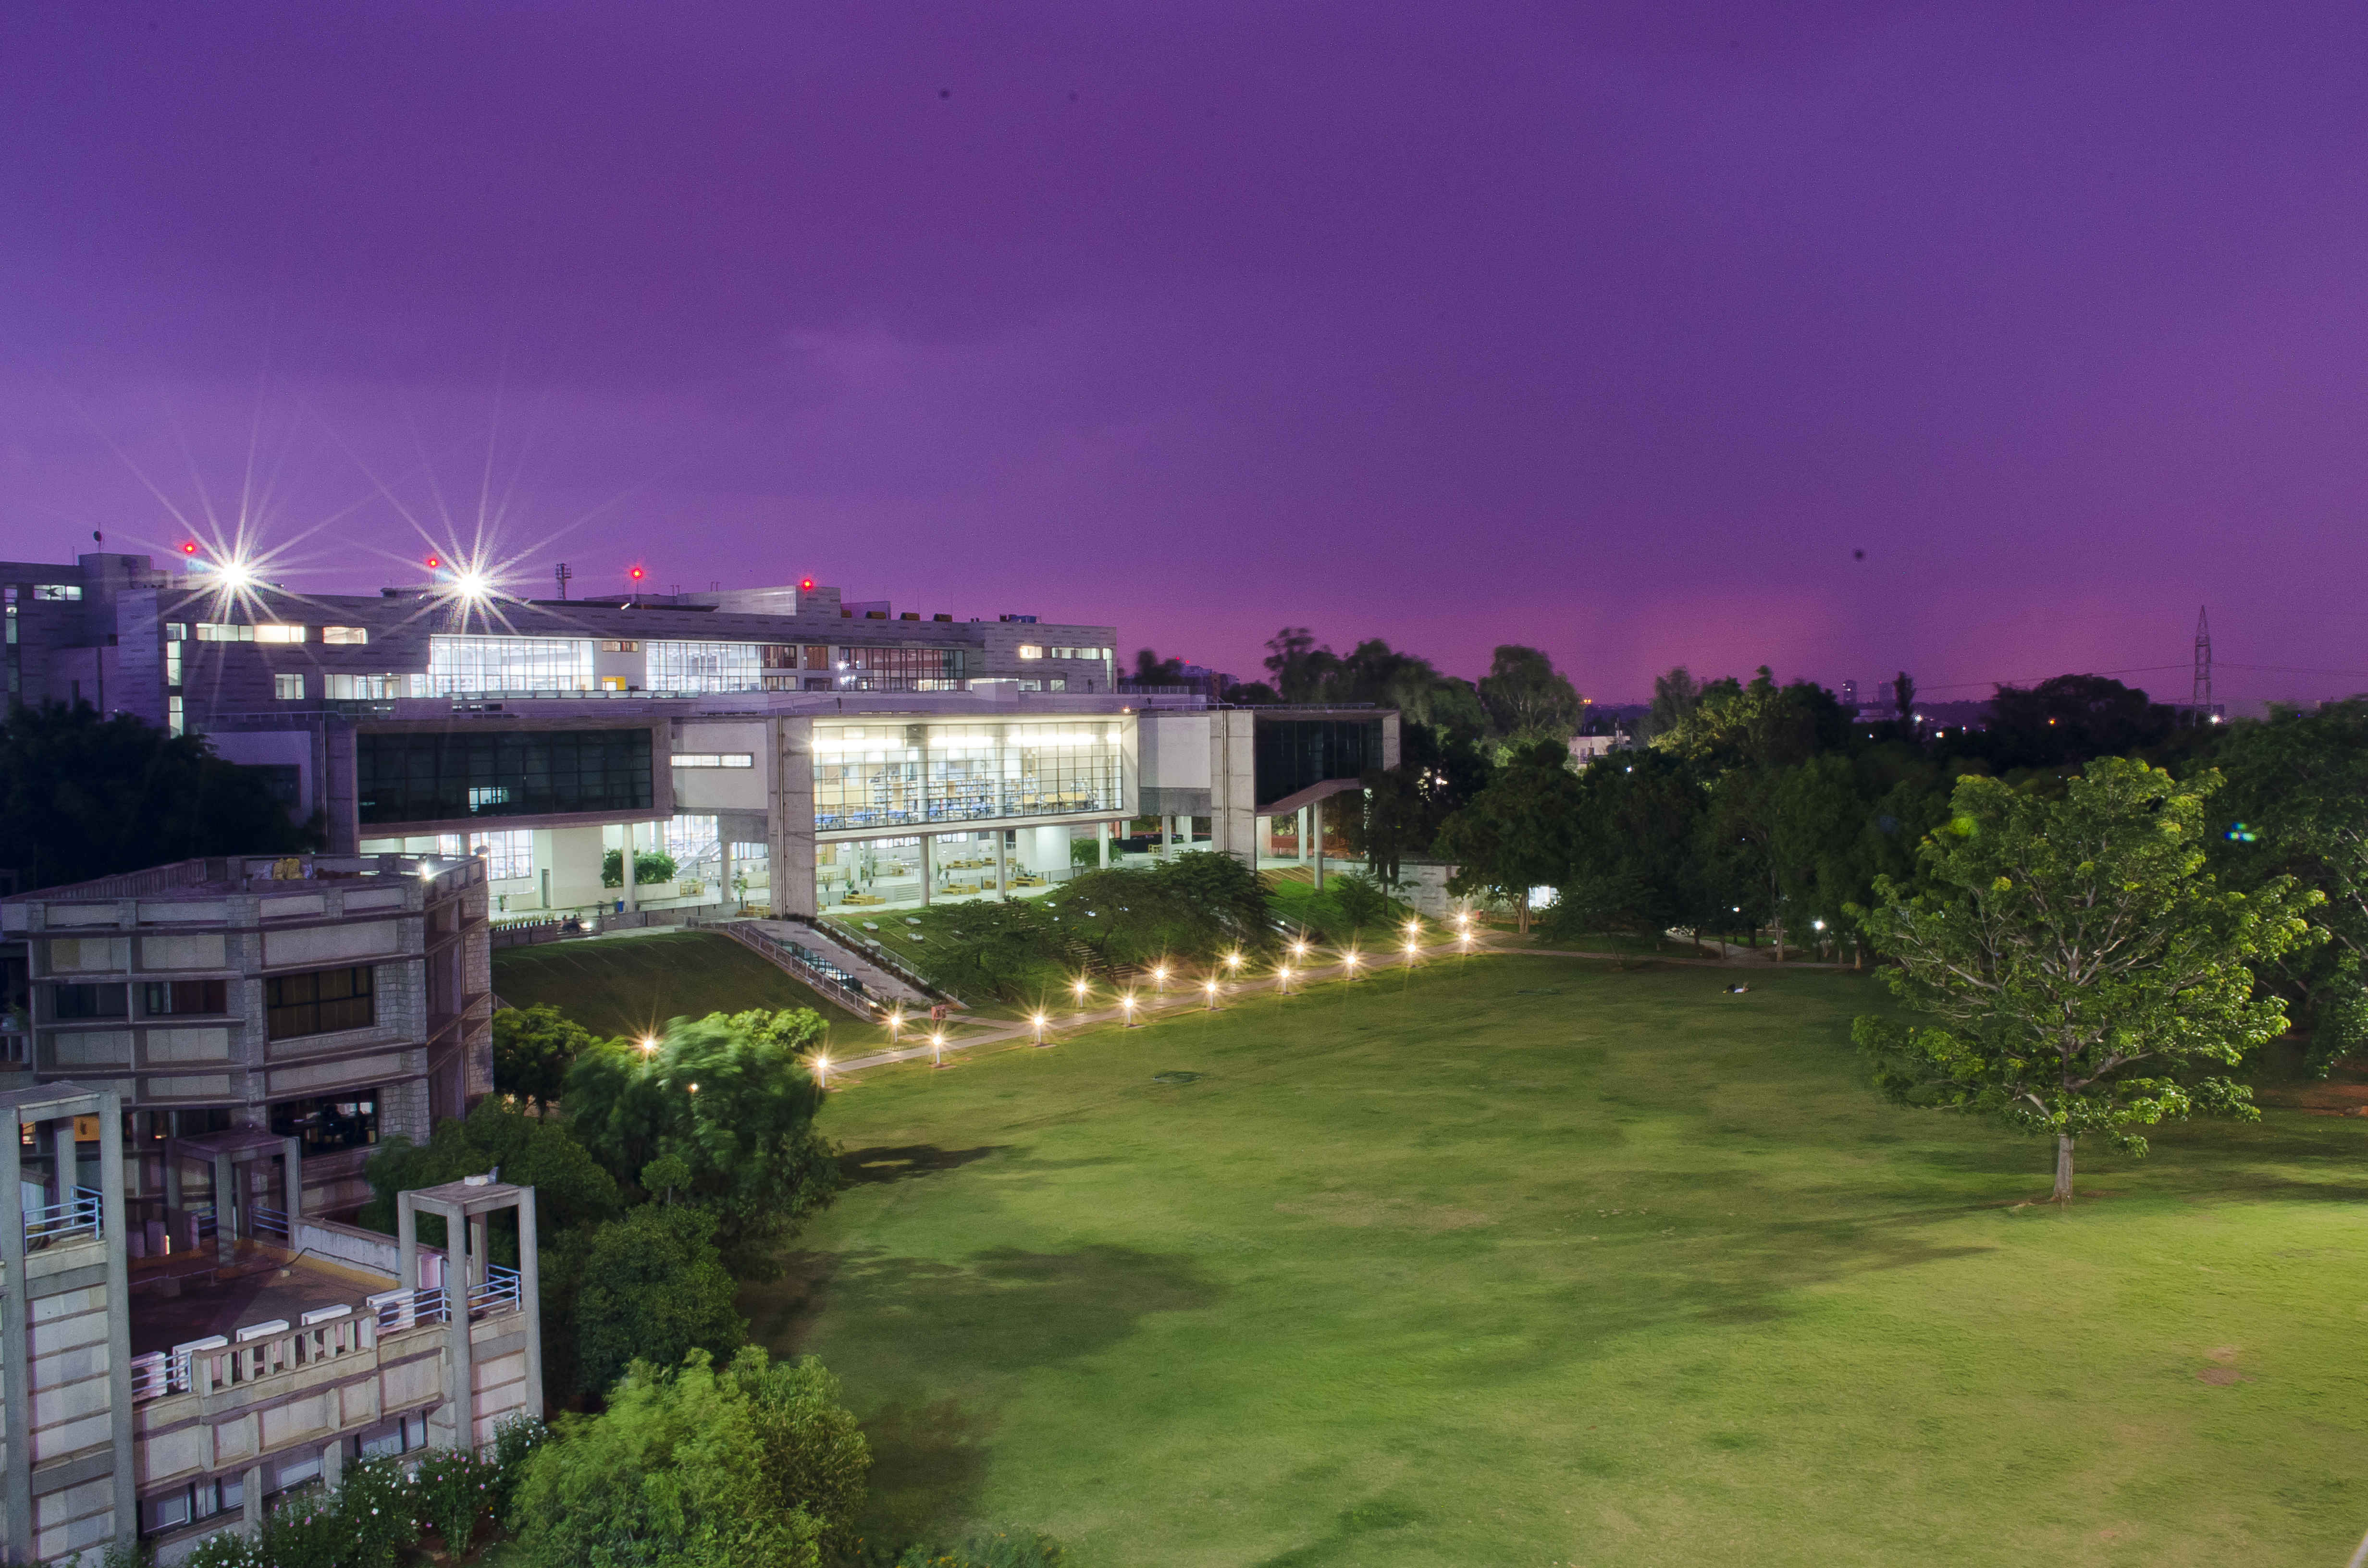
\includegraphics[
            %width=\paperwidth,
            height=\paperheight]{./images/background_low_res.jpg}
    };

    \node[text width=0.6\paperwidth] (title) at (0.45\paperwidth,0) { 
        {\fontsize{1cm}{1.5cm}\selectfont \hfill Student Handbook - 2017}
    };

    \node[text width=0.6\paperwidth, below=of title ] (ncbs) {
        {\raggedleft \hfill \Large NCBS Bangalore}
    };
    
    % credit
    \node[inner sep=2pt,yshift=2mm,xshift=3cm] (credit) at (current page.south west)
    {
        \small \tt Image credit : XXXXXXXXXXXXXXXXXXXXXXXXXXXXXXXXXXXXXXXXX
    };

\end{tikzpicture}    


\end{document}
